\documentclass[conference]{IEEEtran}
% \IEEEoverridecommandlockouts
% The preceding line is only needed to identify funding in the first footnote. If that is unneeded, please comment it out.
\usepackage{cite}
\usepackage{amsmath,amssymb,amsfonts}
\usepackage{algorithmic}
\usepackage{graphicx}
\usepackage{textcomp}
\usepackage{xcolor}
\def\BibTeX{{\rm B\kern-.05em{\sc i\kern-.025em b}\kern-.08em
    T\kern-.1667em\lower.7ex\hbox{E}\kern-.125emX}}
\begin{document}

\title{Applications of anomaly detection techniques to intrusion detection}

\author{\IEEEauthorblockN{Christian Westbrook}
\IEEEauthorblockA{\textit{Department of Computer Science} \\
\textit{Colorado State University}\\
Fort Collins, U.S.A. \\
christian.westbrook@colostate.edu}}

\maketitle

\begin{abstract}
Intrusion detection is a common cybersecurity task involving the inspection of a networked environment for evidence of malicious activity. One approach to intrusion detection is to view the problem as a need to identify anomalous network activity. In this work we demonstrate that idea by performing a series of experiments applying known machine learning techniques for anomaly detection to an intrusion detection task. We employ the CICIDS2017 dataset of labeled network intrusion events in the training of our models. We set out to compare the effectiveness of multiple anomaly detection techniques in the task of identifying malicious packet events from the given dataset. To this end we experiment with applications of Mahalanobis distances, K-Nearest Neighbors, Local Outlier Factor, Isolation Forests, Multiple Linear Regression, and Principal Component Analysis to the network intrusion task. We found that models operating under the assumption that anomalies exist at a distance from normal data points scored poorly in recall while models operating under the assumption that anomalies exist in low density regions of the state space scored well in recall. We also discovered that most of our models struggled with precision, triggering an excessively high number of false alarms.
\end{abstract}

\begin{IEEEkeywords}
anomaly detection, intrusion detection, k-nearest neighbors, 
\end{IEEEkeywords}

\section{Introduction}

Intrusion detection is a common cybersecurity task involving the inspection of a networked environment for evidence of malicious activity. One approach to intrusion detection is to view the problem as a need to identify anomalous network activity. This point of view allows for the application of a number of well-known techniques from the rich and varied field of anomaly detection to intrusion detection tasks. In this work we demonstrate that idea by performing a series of experiments applying known anomaly detection techniques to an intrusion detection task.

Our objective is to compare multiple anomaly detection techniques in how effectively they can identify anomalous network traffic. We chose to employ the CICIDS2017 dataset of labeled network intrusion events to train our models for the task of identifying malicious packet events in a network. We chose to test a series of anomaly detection techniques that will each make a different assumption about the nature of anomalous data in a dataset. The practice of applying multiple anomaly detection techniques to the same task allows an analyst to potentially draw conclusions about the nature of the anomalous data in their particular scenario. To this end we experiment with applications of Mahalanobis distances, K-Nearest Neighbors, Local Outlier Factor, Isolation Forests, Multiple Linear Regression, and Principal Component Analysis to our network intrusion task.

This work continues with a description of the CICIDS2017 dataset and then of the experiments that we performed. This is followed by an evaluation and analysis of the outcomes of our experiments before concluding with a discussion of potential avenues for future work.

\section{Data}

To train a set of machine learning models for the task of identifying malicious packet events in a network we needed a labeled dataset of both benign and malicious packet events. A labeled dataset greatly simplifies the effort required in evaluating model performance while also opening the door to supervised learning techniques. This dataset should be large enough to serve as a suitable input to our models while remaining small enough to be processed in a realistic amount of time.

We chose to use the CICIDS2017 dataset of network intrusion events, developed by the Canadian Institute for Cybersecurity and the University of New Brunswick, because it meets all of these needs. This dataset is a collection of both real and simulated packet capture events that are labeled as either benign or attack events. The authors of the dataset established both a victim network and an attack network, each being a complete network topology consisting of routers, firewalls, switches, and end-user machines. The authors use a machine-learning tool called B-Profile to generate simulated benign network activity for the dataset across a period of five consecutive days, during which time the authors also launch a series of attacks against the victim network from the attack network. All network traffic that passed through the victim network during this time period was captured and labeled. The result is a dataset of just over 2,800,000 packet capture events with 79 features, including 77 numerical features like 'Flow Duration' and 'Fwd Packets/s', along with two categorical fields, namely the 'Destination Port' and the 'Label'.

During our preprocessing step we wanted to prepare the dataset to serve as input into a binary classification task for anomaly detection rather than for a multi-class classification task. This led us to the decision to simplify our dataset's labeling by encoding all instances of the label 'BENIGN' into the value 0 and all instances of any other labels, representing various kinds of attack events, into the value 1. This format allowed our labels to better serve their purpose as targets during the training and evaluation of our models. We then separated the labels from the rest of the dataset.

\section{Methods}

In this section we detail the exact machine learning techniques used for anomaly detection in each of our seven experiments. In every case the goal of the model is to accurately predict which data points are anomalous. This is analogous to the model detecting which packet capture events represent attacks on the victim network. In each experiment we consider how the assumptions made by the given technique will impact its ability to find anomalies, split our data into training and test sets, build the model described in the experiment details, and make predictions against the test set for evaluation.

\subsection*{Experiment 1: Mahalanobis Distance}

In our first experiment we employ a technique that uses a point's proximity to the distribution of points in the dataset as a mechanism for detecting anomalies. The Mahalanobis distance of a point represents its distance from the given distribution. Using a vector of sample means and a vector of sample standard deviations computed from the training set we generate a centerpoint for the distribution. We then use the covariance matrix of the dataset's features to control the shape of the distribution around the centerpoint when computing Mahalanobis distances for each point in the test set. We finally establish a threshold distance away from the distribution beyond which any point is labeled an anomaly. This technique makes the assumption that an anomalous point is further away from the distribution than normal points.

In our implementation of this experiment we performed a grid search of the hyperparameter space of the cutoff threshold.

\subsection*{Experiment 2: Isolation Forest}

In this experiment we employ a technique that takes advantage of the idea that anomalies are few in number and distant from normal data points, thus making them easier to isolate. The isolation forest algorithm repeatedly selects a feature at random and then selects a random value for that feature within the range of allowable values, dividing the data along that random value for the given random feature and thereby partitioning the data at that point. The repeated process of partitioning smaller and smaller regions of space can be considered from the perspective of a tree structure, with leaves representing the smaller partitions produced by each division. This process occurs in a hierarchical fashion, with partitions of space at the same distance from the root node of the isolation tree being divided before partitions at lower levels.

At some point in this process every point will exist within its own partition, and a length can be computed from the root node to the isolating leaf to determine how many partitioning steps were required to isolate a given point. Points that are successfully isolated in fewer steps are then considered anomalous based on the assumption that anomalies are inherently easier to isolate. This algorithm makes the assumption that an anomalous point will be easier to isolate using random hierarchical partitioning.

In our implementation of this experiment we performed a grid search of the hyperparameter space of the number of trees to be used.

\subsection*{Experiment 3: Multiple Linear Regression}

In this experiment we employ a very traditional technique for classification tasks that uses a linear model as a mechanism for detecting anomalies. The linear regression algorithm begins generating a linear model of the data by choosing a line at random. It then iterates by making small adjustments to the model based on the proximity of the line to each of the points in the dataset, attempting to minimize a squared error cost function in order to achieve the best possible fit to the training data. New points can be plotted against the linear model to generate predictions about their labels, represented by the Y axis of the linear model. This technique assumes that a linear model can portray the relationship between sample features and their labels.

\subsection*{Experiment 4: Principal Component Analysis and K-Nearest Neighbors}

In this experiment we employ both a technique for dimensionality reduction and a technique for anomaly detection.

First we employ a technique for dimensionality reduction called Principal Component Analysis that, at a high level, uses the variance of each feature to determine which features are more important than others and to generate a lower dimensional view of the data consisting of linear transformations of features deemed to be the most import. This technique makes the assumption that features with greater variance are the most important.

Next we employ a technique that uses the labels of other points in proximity to a given point to determine whether it is anomalous. The K-Nearest Neighbors algorithm computes the Euclidean distances from a given point to all other points in a dataset to determine its nearest neighbors. The algorithm will then poll the class labels of the given point's k nearest neighbors, using the majority occurrence to predict the label of the new point. Dimensionality reduction is important when making use of this algorithm as a way to greatly reduce the temporal complexity of both training and making predictions. This technique makes the assumption that an anomalous point is close to other anomalies, which is not necessarily true for every dataset.

In our implementation of this experiment we performed a grid search of the hyperparameter space of the number of neighbors to be polled when making predictions.

\subsection*{Experiment 5: Principal Component Analysis and Local Outlier Factor}

In this experiment we employ both a technique for dimensionality reduction and a technique for anomaly detection.

First we employ Principal Component Analysis for dimensionality reduction, which was described previously in the Experiment 5 subsection. Next we employ a technique that uses the local density surrounding a point as a mechanism for detecting anomalies. The local outlier factor of a point is a measure of local density estimated using the distances from a given point to its k nearest neighbors. A lower local outlier factor will correspond to a point existing in a lower density region of the state space. Dimensionality reduction is important when making use of this algorithm as a way to greatly reduce the temporal complexity of both training and making predictions.  This technique makes the assumption that an anomalous point will exist in a lower density region of the state space.

In our implementation of this experiment we performed a grid search of the hyperparameter space of the number of neighbors to be used in density calculations.

\begin{figure}[htbp]
\centerline{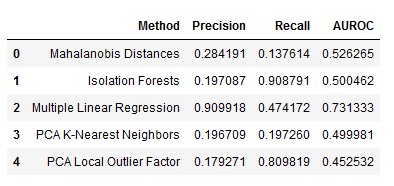
\includegraphics{results.png}}
\caption{Performance metrics across all experiments.}
\label{fig}
\end{figure}

\section{Evaluation}

For the evaluation of our models we have collected a series of three metrics, being precision, recall, and AUROC. As it relates to our intrusion detection task specifically, the recall metric is the most important to maximize. The primary goal of our task is to detect as many of the anomalies as possible to prevent attacks from causing damage to a system. With this in mind, it is made clear by our performance metrics that the Isolation Forest algorithm was the best at detecting anomalies, boasting a recall of 90.9\%. The Local Outlier Factor method comes in second at a respectable 81.0\% while the other three methods come up short.

The methods with the lowest recall, being the Mahalanobis Distance method and the K-Nearest Neighbors method, tell us something about the nature of anomalous points in our dataset. These scores imply that malicous packet events occur in relatively close proximity to the distribution of packet events, and that the nearest neighbors to a malicious event plotted in our dataset's state space are often benign events rather than anomalies. This is an interesting characteristic in that the anomalies are apparently able to blend in, to some extent, with normal events.

On the contrary, our two highest recall methods can also shed some light on the nature of our anomalous data. The Local Outlier Factor method relies directly on low local area densities to detect anomalies while the Isolation Forest method indirectly uses local area density to isolate anomalies in fewer steps than normal data. This implies that even if our network intrusion events occur in close proximity to benign events, they often tend to occur in areas of low density. This is a useful characteristic of malicious events to extract from these metrics.

Taking a look at the precision column of our metric table reveals that most of our models produced a problematic number of false alarms. Even the Isolation Forest model with its impressive recall suffers from a precision of only 19.7\%. This indicates that our best models have room to grow with additional refinement and tuning.

It's very interesting to note the one model that was able to attain a high level of precision along with a recall that isn't quite as abysmal as it is for other models. The Multiple Linear Regression model achieved a precision of 91.0\% and a recall of 47.4\%. Looking at the AUROC metrics for each of our models, we can see that the Multiple Linear Regression model comes away with the best combined performance. This is promising. The intuitive next step beyond linear regression is the artificial neural network, and with these results my next step would be to try training a neural network for this task.

\section{Conclusion}

Machine learning techniques for anomaly detection can perform well on intrusion detection tasks. An analysis of our model performance indicates that attacks on our victim network are located in close proximity to benign network traffic events within the state space of our dataset, but that they tend to lie in regions of low density and that his characteristic can be exploited by certain types of models to detect anomalies with a high rate of recall. We also discovered that most of our models trigger an unsustainable number of false alarms and would require additional refinement.

Further work in this area should not only continue to refine the existing models defined here, but would also attempt to apply new types of models to the same task. One such model that seems likely to be applied successfully is the artificial neural network. Another interesting type of model that might be fruitful when applied to our specific task would be an angle-based model. This model would compute the angles between a new point and pairs of its k nearest neighbors, using the assumption that points with smaller angles measured in such a manner are more likely to be anomalies. This may work well with the given dataset due to the tendency for anomalous points to exist in low density regions of the state space.

\bibliographystyle{ieeetran}
%\bibliography{IEEEexample}

\begin{thebibliography}{00}
\bibitem{b1} Cansiz, S. (2021, April 17). Multivariate Outlier Detection in Python. Medium. https://towardsdatascience.com/multivariate-outlier-detection-in-python-e946cfc843b3. 
\bibitem{b2} Harris, C. R., Millman, K. J., Walt, S. J. van der, Gommers, R., Virtanen, P., Cournapeau, D., … Oliphant, T. E. (2020, September 16). Array programming with NumPy. Nature News. https://www.nature.com/articles/s41586-020-2649-2. 
\bibitem{b3} Pasricha, S. (2020, November). Anomaly Detection and Security. Embedded Systems and Machine Learning. Fort Collins, CO; Colorado State University. 
\bibitem{b4} Pedregosa, F., Profile, V., Varoquaux, G., Gramfort, A., Michel, V., Thirion, B., … Authors:   Fabian Pedregosa  View Profile. (2011, November 1). Scikit-learn: Machine Learning in Python. The Journal of Machine Learning Research. https://dl.acm.org/doi/10.5555/1953048.2078195. 
\bibitem{b5}Sharafaldin, I., Habibi Lashkari, A., \& Ghorbani, A. A. (2018). Toward Generating a New Intrusion Detection Dataset and Intrusion Traffic Characterization. Proceedings of the 4th International Conference on Information Systems Security and Privacy. https://doi.org/10.5220/0006639801080116 
\bibitem{b6}Virtanen P;Gommers R;Oliphant TE;Haberland M;Reddy T;Cournapeau D;Burovski E;Peterson P;Weckesser W;Bright J;van der Walt SJ;Brett M;Wilson J;Millman KJ;Mayorov N;Nelson ARJ;Jones E;Kern R;Larson E;Carey CJ;Polat İ;Feng Y;Moore EW;VanderPlas J;Laxalde D;P. (n.d.). SciPy 1.0: fundamental algorithms for scientific computing in Python. Nature methods. https://pubmed.ncbi.nlm.nih.gov/32015543/. 
\end{thebibliography}

\end{document}
